\documentclass[12pt]{beamer}


\usepackage[brazilian]{babel}
\usepackage[T1]{fontenc}
\usepackage[utf8]{inputenc}
\usepackage{amsmath,amsfonts,graphicx}
\usepackage{pslatex}
\usepackage{caption}
\usepackage{animate}

\usepackage{ragged2e}
\usepackage{tikz}

\usetikzlibrary{matrix,backgrounds}
\usepackage{parselines} 

\usepackage{multirow}
\usepackage{booktabs}

%\usepackage{minipage}
\usepackage{subfigure}
\usepackage{graphicx}

\usepackage{gensymb}


\usepackage{caption}

\usepackage{etoolbox}
\usepackage{tikzscale}
\usepackage{tikzinclude}

%================

\usepackage{array}

\definecolor{FireBrick}{rgb}{0.7, 0.13, 0.13}
\definecolor{OrangeRed}{rgb}{1.0, 0.27, 0.0}
\definecolor{Red}{rgb}{1.0, 0.0, 0.0}

%\usepackage[dvipsnames]{xcolor} 

\usetikzlibrary{fadings,shapes.arrows,shadows}  
\usepackage{xparse}

\usepackage{lipsum} 

\tikzfading[name=arrowfading, top color=transparent!0, bottom color=transparent!95]
\tikzset{arrowfill/.style={#1,general shadow={fill=black, shadow yshift=-0.8ex, path fading=arrowfading}}}
\tikzset{arrowstyle/.style n args={3}{draw=#2,arrowfill={#3}, single arrow,minimum height=#1, single arrow,
single arrow head extend=.3cm,}}

\NewDocumentCommand{\tikzfancyarrow}{O{2cm} O{FireBrick} O{top color=OrangeRed!20, bottom color=Red} m}{
\tikz[baseline=-0.5ex]\node [arrowstyle={#1}{#2}{#3}] {#4};
}
%================
\usetikzlibrary{arrows, decorations.markings}

% for double arrows a la chef
% adapt line thickness and line width, if needed
\tikzstyle{vecArrow} = [thick, decoration={markings,mark=at position
   1 with {\arrow[semithick]{open triangle 60}}},
   double distance=1.4pt, shorten >= 5.5pt,
   preaction = {decorate},
   postaction = {draw,line width=1.4pt, white,shorten >= 4.5pt}]
\tikzstyle{innerWhite} = [semithick, white,line width=1.4pt, shorten >= 4.5pt]


%================

% Specify theme
\usetheme{UnofficialUChicago}



 %\setbeamertemplate{footline}[frame number]{} % Uncomment this line if you want to remove the footer from each slide (and replace it with just the slide number (X/Y) in the bottom right of each slide.

%===============================================================%
% 				BEGIN YOUR PRESENTATION HERE					%
%===============================================================%
%\justifying
% Title and author information
\title[Introdução a Git e Github]{\centering Introdução ao Git e Github}
%\subtitle{Uma Abordagem Computacional}
\author[Cristian Tiago E. Mendes]{Cristian Tiago Erazo Mendes\\
  %\href{Doutorando em Estatística - UFLA}{{\tt {\scriptsize Doutorando em Estatística e Experimentação Agropecuária - UFLA}}}
  }
\institute[]{Universidade Federal de Lavras}
\date{\today}


%  \usepackage[sfmath]{kpfonts}
%  \renewcommand*\familydefault{\sfdefault}

%\setbeamerfont{frametitle}{shape=\scshape}

%===============================================================%
\begin{document}
%===============================================================%

\maketitle

%%===============================================================%
%\begin{frame}{Sumário}{}
%\tableofcontents
%\end{frame}

%===============================================================%
\footnotesize
\justifying


%===============================================================%

%\section{Sistema de Controle de versão}
\begin{frame}{O que é controle de versão?}
	\begin{figure}[!htb]
		\centering
		%\caption{\scriptsize Exemplo de Entropia.} %legenda
		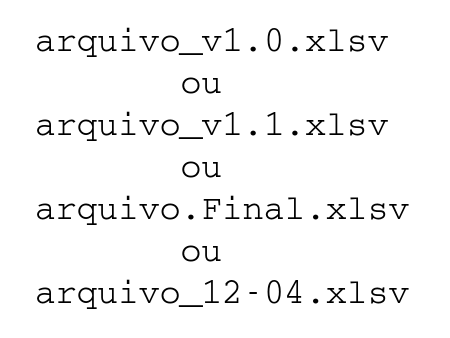
\includegraphics[scale=0.5]{figuras/fig1.png} 
		\label{fig:fig1} %rotulo para refencia
	\end{figure}
\end{frame}

%===============================================================%

\begin{frame}{Onde posso usar controle de versão?}
	\begin{figure}[!htb]
		\centering
		%\caption{\scriptsize Exemplo de Entropia.} %legenda
		
\includegraphics[scale=0.35]{figuras/fig2.png} 
		\label{fig:fig1} %rotulo para refencia
	\end{figure}

\end{frame}


%===============================================================%
\begin{frame}{Onde posso usar controle de versão?}
	\begin{figure}[!htb]
		\centering
		%\caption{\scriptsize Exemplo de Entropia.} %legenda
		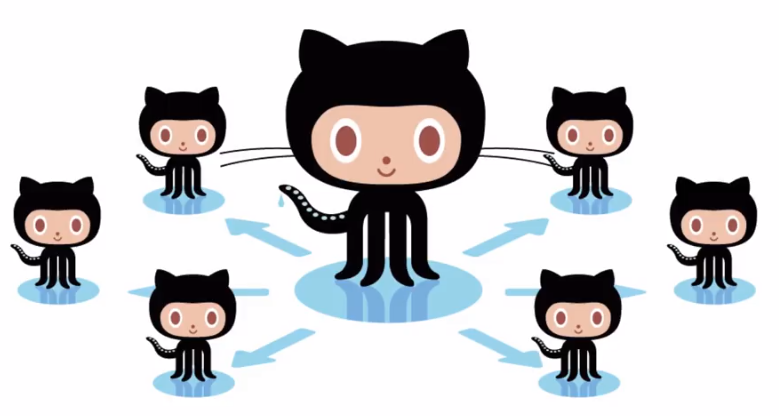
\includegraphics[scale=0.4]{figuras/fig3.png} 
		\label{fig:fig1} %rotulo para refencia
	\end{figure}

\end{frame}
%===============================================================%


\begin{frame}{Onde posso usar controle de versão?}
 \begin{itemize}
 \item Trabalhos de faculdade,
 \item Projetos de desenvolvimento de códigos fontes,
 \item Trabalhos que utilizam word,
 \item Trabalhos de conclusão de curso, dissertações e teses.
 \end{itemize}
\end{frame}

%===============================================================%


%\section{Sistema de Controle de versão}

\begin{frame}{O que é um sistema de controle de versão? }
	\begin{itemize}
		\item É um sistema que registra alterações em um arquivo ou conjunto de arquivos ao longo do tempo,
		\item Permite reverter arquivos ou projetos selecionados para um estado anterior,
		\item Compare as alterações ao longo do tempo,
		\item Recuperar arquivos que foram deletados ou corrompidos,
		\item Podem ser classificados como locais, centralizados ou distribuidos. 
	\end{itemize}
\end{frame}

%===============================================================%

\begin{frame}{Sistemas de Controle de Versão Local}
	\begin{columns}
	    \begin{column}{0.5\textwidth}  %%<--- here
	      \begin{center}
		 		Sistemas de Controle de Versão Local possuem um banco de dados simples que mantem todas as alterações nos arquivos sob controle de revisão.
			\end{center}
	    \end{column}\begin{column}{0.5\textwidth}
			\begin{figure}[!htb]
      		\centering
            %\caption{\scriptsize Exemplo de desequilíbrio de ligação.} %legenda
            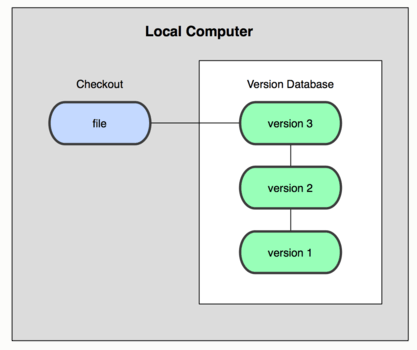
\includegraphics[scale=0.4]{figuras/fig7.png} 
            %\label{fig:reproducao_afideos} %rotulo para refencia
         \end{figure}
	    \end{column}
	    
	\end{columns}
\end{frame}

%===============================================================%
\begin{frame}{Sistemas de Controle de Versão Centralizados}
	\begin{columns}
	    \begin{column}{0.5\textwidth}  %%<--- here
	      \begin{center}
	      		\justifying
		 		 Esses sistemas possuem um único servidor que contém todos os arquivos com versão e um número de clientes que fazem o check-out dos arquivos daquele local central, alguns exemplos são CVS, Subversion e Perforce.
			\end{center}
	    \end{column}\begin{column}{0.5\textwidth}
			\begin{figure}[!htb]
      		\centering
            %\caption{\scriptsize Exemplo de desequilíbrio de ligação.} %legenda
            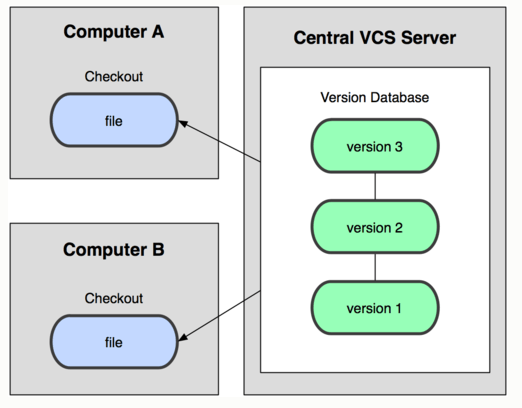
\includegraphics[scale=0.4]{figuras/fig6.png} 
            %\label{fig:reproducao_afideos} %rotulo para refencia
         \end{figure}
	    \end{column}
	    
	\end{columns}
\end{frame}

%===============================================================%
\begin{frame}{Sistemas de Controle de Versão Distribuidos}
	\begin{columns}
	    \begin{column}{0.5\textwidth}  %%<--- here
	      \begin{center}
	      		\justifying
		 		Em um SCV distribuido, os clientes não apenas checam o último registro dos arquivos; em vez disso, elas espelham totalmente o repositório, incluindo seu histórico completo. Possui vários repositórios autônomos e independentes, um para cada cliente, para que você possa colaborar com diferentes grupos de pessoas de diferentes maneiras simultaneamente dentro do mesmo projeto. Alguns exemplos de sistemas são Git, Mercurial, Bazaar ou Darcs.
			\end{center}
	    \end{column}\begin{column}{0.5\textwidth}
			\begin{figure}[!htb]
      		\centering
            %\caption{\scriptsize Exemplo de desequilíbrio de ligação.} %legenda
            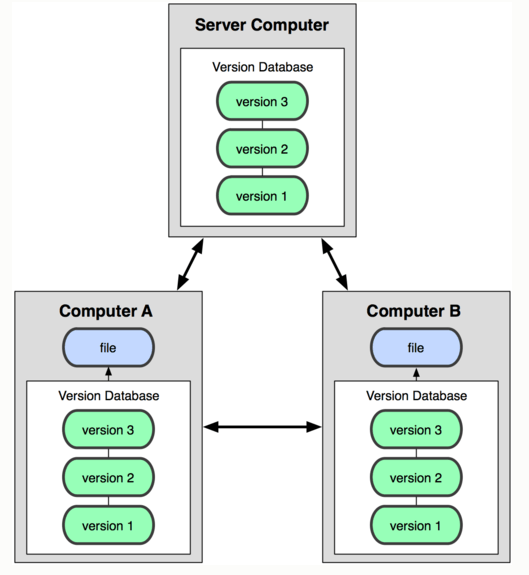
\includegraphics[scale=0.4]{figuras/fig8.png} 
            %\label{fig:reproducao_afideos} %rotulo para refencia
         \end{figure}
	    \end{column}
	    
	\end{columns}
\end{frame}

%===============================================================%
\begin{frame}{Sistema de controle de versão - Git}
	\begin{figure}[!htb]
		\centering
		%\caption{\scriptsize Exemplo de Entropia.} %legenda
		
\includegraphics[scale=0.15]{figuras/git.png} 
		\label{fig:git} %rotulo para refencia
	\end{figure}
	\begin{itemize}
		\item Sistema de controle de arquivo,
		\item Possui o controle do dominio do histórico mudanças nos arquivos,		
		\item Faz todo gerenciamento do processo de desenvolvimento do projeto.
	\end{itemize}
\end{frame}

%===============================================================%

\begin{frame}{Sistema de controle de versão - Git}

	\begin{columns}
	    \begin{column}{0.5\textwidth}  %%<--- here
	      \begin{center}
	      		\justifying


Git surgiu a partir de um projeto de software de código aberto, o kernel (núcleo) do Linux, em que durante o período de manutenção do kernel (1991-2002), as mudanças no software eram repassadas como patches e arquivos compactados. Em 2002, passou a utilizar no projeto um sistema DVCS proprietário chamado BitKeeper. Em 2005, a parceria desfez, e isso levou a comunidade de desenvolvedores do Linux a desenvolver sua própria ferramenta.

			\end{center}
	    \end{column}\begin{column}{0.5\textwidth}
			 \hspace{2.5mm} Linus Torvalds (criador do Linux):\\			
			\begin{figure}[!htb]
      		\centering
            %\caption{\scriptsize Exemplo de desequilíbrio de ligação.} %legenda
            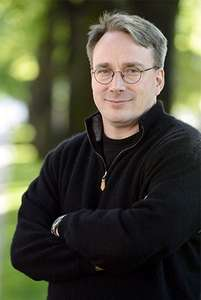
\includegraphics[scale=0.4]{figuras/linust.jpg} 
            %\label{fig:reproducao_afideos} %rotulo para refencia
         \end{figure}
	    \end{column}
	    
	\end{columns}
  
\end{frame}

%===============================================================%

\begin{frame}{Sistema de controle de versão - Git}

	\begin{figure}[!htb]
		\centering
		%\caption{\scriptsize Exemplo de Entropia.} %legenda
		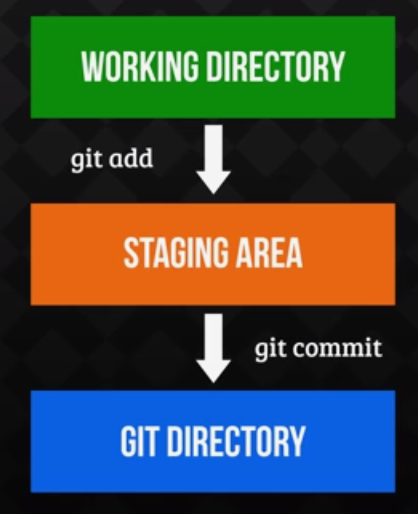
\includegraphics[scale=0.45]{figuras/fig5.png} 
		\label{fig:fig1} %rotulo para refencia
	\end{figure}
	\centering \url{https://git-scm.com/}
\end{frame}

%===============================================================%

\begin{frame}{o que é Github?}
	\begin{figure}[!htb]
    	\centering
        %\caption{\scriptsize Exemplo de desequilíbrio de ligação.} %legenda
		
\includegraphics[scale=0.5]{figuras/github.png} 
		%\label{fig:reproducao_afideos} %rotulo para refencia
	\end{figure}
	\begin{itemize}
		\item Plataforma de guarda repositórios criados pelo git,
		\item Acesso remoto dos projetos em desenvolvimento.
	\end{itemize}
	\centering \url{https://github.com}
	
\end{frame}

%===============================================================%


\begin{frame}{o que é Github?}
	\begin{figure}[!htb]
    	\centering
        %\caption{\scriptsize Exemplo de desequilíbrio de ligação.} %legenda
		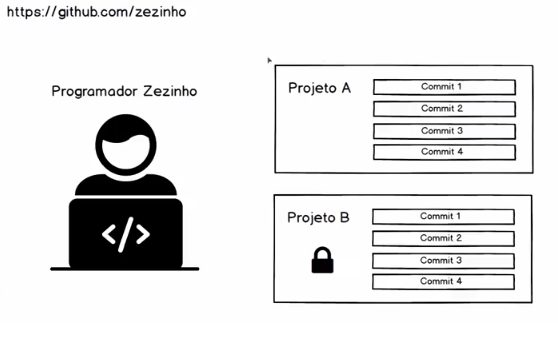
\includegraphics[scale=0.5]{figuras/fig9.png} 
		%\label{fig:reproducao_afideos} %rotulo para refencia
	\end{figure}
\end{frame}

%===============================================================%


\begin{frame}{o que é Github?}
	\begin{figure}[!htb]
    	\centering
        %\caption{\scriptsize Exemplo de desequilíbrio de ligação.} %legenda
		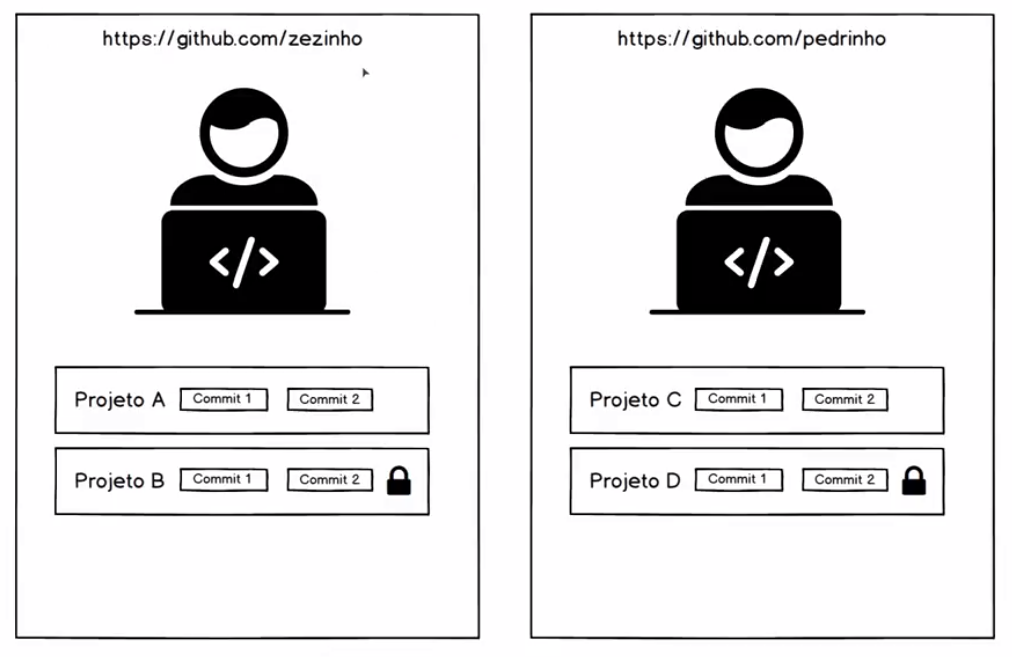
\includegraphics[scale=0.3]{figuras/fig10.png} 
		%\label{fig:reproducao_afideos} %rotulo para refencia
	\end{figure}
\end{frame}

%===============================================================%


\begin{frame}{o que é Github?}
	\begin{figure}[!htb]
    	\centering
        %\caption{\scriptsize Exemplo de desequilíbrio de ligação.} %legenda
		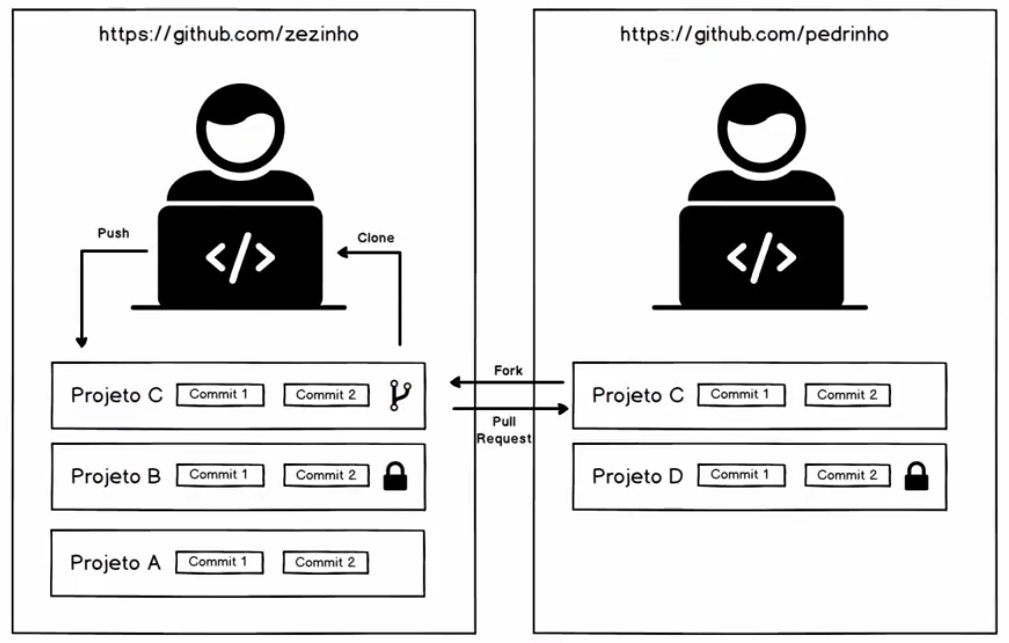
\includegraphics[scale=0.3]{figuras/fig11.png} 
		%\label{fig:reproducao_afideos} %rotulo para refencia
	\end{figure}
\end{frame}

%===============================================================%

\begin{frame}{Utilizando interface para Github}
	\begin{figure}[!htb]
    	\centering
        %\caption{\scriptsize Exemplo de desequilíbrio de ligação.} %legenda
		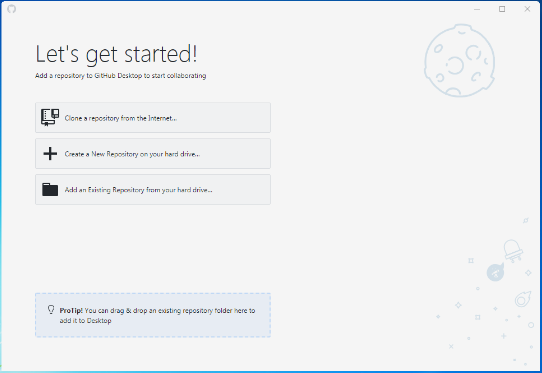
\includegraphics[scale=0.7]{figuras/fig12.png} 
		%\label{fig:reproducao_afideos} %rotulo para refencia
	\end{figure}
\end{frame}

%===============================================================%

%
%\section{REFERÊNCIAS}
%\begin{frame}{REFERÊNCIAS}
%\begin{itemize}
%
%\item 
%
%\end{itemize}
%\end{frame}

%===============================================================%
{
\BackgroundShaded
\section{}
\begin{frame}[noframenumbering]
\centering
%\textcolor{white}{\Huge Obrigado!}
\textcolor{white}{\resizebox{!}{1cm}{Obrigado!}}
\end{frame}
}


%===============================================================%
\end{document}
%===============================================================% 
\grid
